\documentclass[12pt, a4paper]{article}

% Packages
\usepackage[utf8]{inputenc}
\usepackage[T1]{fontenc}
\usepackage{lmodern}
\usepackage[margin=1in]{geometry}
\usepackage{graphicx}
\usepackage{hyperref}
\usepackage{listings}
\usepackage{xcolor}
\usepackage{booktabs}
\usepackage{caption}
\usepackage{float}
\usepackage{amsmath}
\usepackage{enumitem}
\usepackage{fancyhdr}
\usepackage{tikz}
\usetikzlibrary{shapes.geometric, arrows.meta, positioning}

% Code listing style
\definecolor{codebg}{RGB}{245, 245, 245}
\definecolor{codegreen}{RGB}{0, 128, 0}
\definecolor{codegray}{RGB}{128, 128, 128}
\definecolor{codeblue}{RGB}{0, 0, 180}
\definecolor{codered}{RGB}{200, 0, 0}

\lstdefinestyle{pythonstyle}{
    language=Python,
    backgroundcolor=\color{codebg},
    basicstyle=\ttfamily\footnotesize,
    keywordstyle=\color{codeblue}\bfseries,
    stringstyle=\color{codered},
    commentstyle=\color{codegreen}\itshape,
    numberstyle=\tiny\color{codegray},
    numbers=left,
    numbersep=8pt,
    frame=single,
    framerule=0.5pt,
    rulecolor=\color{codegray},
    breaklines=true,
    breakatwhitespace=false,
    tabsize=4,
    showstringspaces=false,
    captionpos=b,
    aboveskip=10pt,
    belowskip=10pt,
}
\lstdefinestyle{plain}{
    language={},
    backgroundcolor=\color{codebg},
    basicstyle=\ttfamily\scriptsize,
    frame=single,
    framerule=0.5pt,
    rulecolor=\color{codegray},
    breaklines=true,
    columns=fullflexible,
    keepspaces=true,
    showstringspaces=false,
    captionpos=b,
}
\lstset{style=pythonstyle}

% Header/Footer
\pagestyle{fancy}
\fancyhf{}
\fancyhead[L]{\small CSE731: Software Testing}
\fancyhead[R]{\small Mid-term Project}
\fancyfoot[C]{\thepage}
\renewcommand{\headrulewidth}{0.4pt}

\hypersetup{
    colorlinks=true,
    linkcolor=blue,
    urlcolor=blue,
    citecolor=blue,
}

% Title
\title{
    \vspace{-1cm}
    \textbf{AI-Assisted Unit Testing Pipeline} \\[0.3cm]
    \large CSE731: Software Testing --- Mid-term Project \\[0.2cm]
    \large Term I (2026--27) \\[0.5cm]
    \normalsize International Institute of Information Technology, Bangalore
}
\author{
    \textbf{Member 1:} Name (Roll Number) \\
    \textbf{Member 2:} Name (Roll Number)
}
\date{September 2026}

\begin{document}

\maketitle
\thispagestyle{fancy}

% ============================================================================
\section{Introduction}

This report presents our AI-assisted unit testing pipeline for the CSE731 Software Testing mid-term project. The pipeline uses a Large Language Model (LLM) to generate a Python function for a programming problem, generates unit test cases (inputs and expected outputs) that satisfy a \textbf{user-specified structural coverage criterion} on that function, validates them against the dataset's reference solution, and executes them to give a verdict.

Of the three test requirements allowed by the assignment (coverage criterion, property, statistical estimation), our pipeline implements \textbf{requirement (1): achieving a user-specified coverage criterion}. The user chooses one of four graph (structural) coverage criteria:
\begin{itemize}
    \item \textbf{Node Coverage} --- every node of the control flow graph (CFG) is executed;
    \item \textbf{Edge Coverage} --- every edge of the CFG is traversed;
    \item \textbf{Edge-Pair Coverage} --- every path of length up to two edges is toured;
    \item \textbf{Prime Path Coverage} (default) --- every prime path is toured.
\end{itemize}

The pipeline is written from first principles in plain Python. It does not use RAG, chain-of-thought prompting or agent frameworks such as LangGraph: every agent is a single, direct LLM call (or deterministic code) and the orchestration is ordinary Python control flow. It consists of three agents:
\begin{enumerate}
    \item \textbf{Code Generator Agent} --- generates one Python function from a natural-language problem description.
    \item \textbf{Test Case Generator Agent} --- generates unit test cases (inputs \emph{and} expected outputs) that achieve the selected coverage criterion on the generated function.
    \item \textbf{Test Executor Agent} --- parses the test cases, checks every test case against the dataset's reference solution (a test case is valid only if the reference solution returns the same expected output), calls the generated function on every valid test case, asserts that its output equals the expected output, and reports a verdict; it also builds the control flow graph of the generated function and verifies whether the test cases achieve the selected coverage criterion.
\end{enumerate}

% ============================================================================
\section{Pipeline Architecture}

\subsection{Overview}

Figure~\ref{fig:pipeline-arch} shows the pipeline. For each problem the three agents run in sequence; the reference solution from the dataset is used only by the Test Executor, to validate the generated test cases.

\begin{figure}[H]
    \centering
    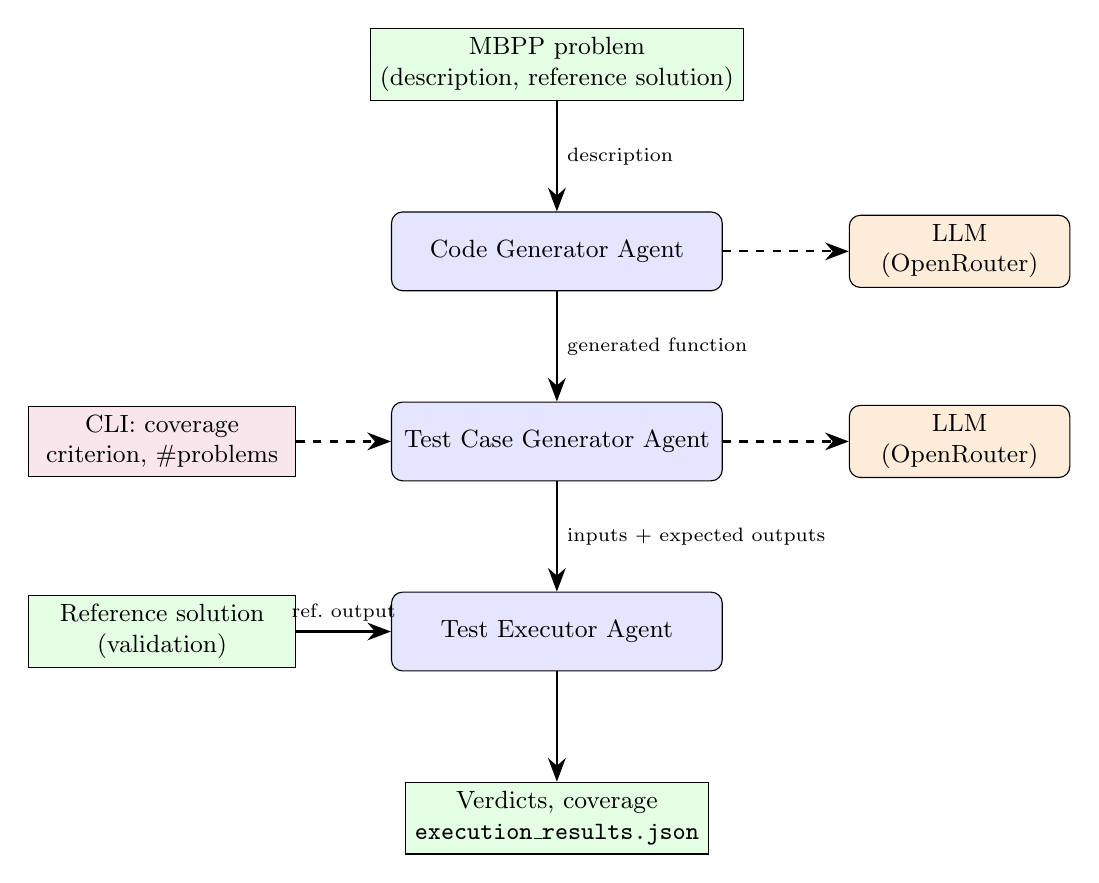
\begin{tikzpicture}[
        node distance=1.4cm,
        block/.style={rectangle, draw, rounded corners, fill=blue!10,
                      minimum width=4.2cm, minimum height=1cm, align=center, font=\small},
        data/.style={rectangle, draw, fill=green!10,
                     minimum width=3.4cm, minimum height=0.8cm, align=center, font=\small},
        llm/.style={rectangle, draw, rounded corners, fill=orange!15,
                    minimum width=2.8cm, minimum height=0.9cm, align=center, font=\small},
        arrow/.style={-{Stealth[length=3mm]}, thick},
    ]
        \node[data] (dataset) {MBPP problem\\(description, reference solution)};
        \node[block, below=of dataset] (codegen) {Code Generator Agent};
        \node[block, below=of codegen] (testgen) {Test Case Generator Agent};
        \node[block, below=of testgen] (executor) {Test Executor Agent};
        \node[data, below=of executor] (results) {Verdicts, coverage\\\texttt{execution\_results.json}};

        \node[llm, right=1.6cm of codegen] (llm1) {LLM\\(OpenRouter)};
        \node[llm, right=1.6cm of testgen] (llm2) {LLM\\(OpenRouter)};
        \node[data, left=1.2cm of executor] (oracle) {Reference solution\\(validation)};
        \node[data, left=1.2cm of testgen, fill=purple!10] (cli) {CLI: coverage\\criterion, \#problems};

        \draw[arrow] (dataset) -- node[right, font=\scriptsize] {description} (codegen);
        \draw[arrow] (codegen) -- node[right, font=\scriptsize] {generated function} (testgen);
        \draw[arrow] (testgen) -- node[right, font=\scriptsize] {inputs + expected outputs} (executor);
        \draw[arrow] (executor) -- (results);
        \draw[arrow, dashed] (codegen) -- (llm1);
        \draw[arrow, dashed] (testgen) -- (llm2);
        \draw[arrow] (oracle) -- node[above, font=\scriptsize] {ref.\ output} (executor);
        \draw[arrow, dashed] (cli) -- (testgen);
    \end{tikzpicture}
    \caption{Pipeline architecture}
    \label{fig:pipeline-arch}
\end{figure}

\subsection{Dataset: MBPP}

We use the \textbf{MBPP (Most Basic Python Problems)} dataset (\texttt{google-research-datasets/mbpp}, \texttt{full} configuration, \texttt{test} split), loaded with the Hugging Face \texttt{datasets} library. Each problem provides:
\begin{itemize}
    \item a natural-language description of the task;
    \item a reference Python solution;
    \item three reference assert statements (used to identify the function name and shown to both LLM agents as example usage).
\end{itemize}
The user chooses how many problems to process (1--50, default 1); problems are taken in dataset order starting from task 11.

\subsection{Flow for One Problem}

\begin{enumerate}
    \item The \textbf{function under test} and its signature (e.g.\ \texttt{remove\_Occ(s, ch)}) are taken from the reference solution; the name is the function called in the dataset's assert statements.
    \item The \textbf{Code Generator} asks the LLM for the function. The response is validated (Section~\ref{sec:codegen}); if invalid, the LLM is asked once more with the reason.
    \item The \textbf{Test Case Generator} asks the LLM for test cases --- inputs and expected outputs --- that achieve the selected coverage criterion on the generated function (Section~\ref{sec:testgen}).
    \item The \textbf{Test Executor} parses the test cases, runs the reference solution on each input to validate the expected output, runs the generated function on every valid test case in a separate process, asserts that its output equals the expected output, and checks whether the valid test cases achieve the selected coverage criterion on the CFG of the generated function (Section~\ref{sec:executor}).
    \item All prompts, raw LLM responses, the generated code, the test cases and the results are written to the \texttt{output/} folder.
\end{enumerate}

\subsection{Technology Stack}

\begin{table}[H]
    \centering
    \begin{tabular}{ll}
        \toprule
        \textbf{Component} & \textbf{Technology} \\
        \midrule
        Language & Python 3 (tested on 3.9 and 3.14) \\
        LLM API & OpenRouter (free models) \\
        CLI & \texttt{argparse} + Rich \\
        Dataset & Hugging Face \texttt{datasets} (MBPP) \\
        Code validation / parsing & Python \texttt{ast} module \\
        Test execution & \texttt{multiprocessing} worker processes with per-test time limit \\
        Coverage verification & CFG built from the AST + recorded test paths \\
        \bottomrule
    \end{tabular}
    \caption{Technology stack}
\end{table}

% ============================================================================
\section{LLM Settings and Parameters}
\label{sec:settings}

Both LLM agents use the same settings. All other sampling parameters (top-p, etc.) are left at the provider defaults.

\begin{table}[H]
    \centering
    \begin{tabular}{ll}
        \toprule
        \textbf{Parameter} & \textbf{Value} \\
        \midrule
        API endpoint & \texttt{https://openrouter.ai/api/v1/chat/completions} \\
        Primary model & \texttt{cohere/north-mini-code:free} \\
        Fallback models & \texttt{google/gemma-4-31b-it:free}, \texttt{google/gemma-4-26b-a4b-it:free}, \\
                        & \texttt{qwen/qwen3.8-27b:free}, \texttt{nvidia/nemotron-3.5-lightning:free}, \\
                        & \texttt{nvidia/nemotron-3-ultra-550b-a55b:free} \\
        Temperature & 0.7 \\
        Max tokens & 4096 \\
        Messages per call & one system message + one user message (no conversation history) \\
        Retries & 1 re-prompt if the response violates the output format (with the rejection reason) \\
        Time limit per test case & 10 seconds \\
        \bottomrule
    \end{tabular}
    \caption{LLM and execution settings}
\end{table}

If the primary model is rate-limited (HTTP 429, retried once after the \texttt{Retry-After} delay) or unavailable (HTTP 404/502/503), the next fallback model is tried. A response that was cut off at the token limit (\texttt{finish\_reason = "length"}) is incomplete and is also discarded in favour of the next model. The model that actually answered is recorded with every response in the output files. Only the model's final answer (\texttt{content}) is used; reasoning/thinking fields returned by some models are ignored.

% ============================================================================
\section{Agent Descriptions and Prompts}

\subsection{Code Generator Agent}
\label{sec:codegen}

\subsubsection{System Prompt}

\begin{lstlisting}[style=plain]
You are a Python code generator in an automated unit-testing pipeline. Your response is loaded by a program that calls your function with test inputs, so it must be exactly one Python 3 function definition and nothing else.

Rules:
1. Write exactly one function, with exactly the name and parameters given in the user message.
2. Put any import statements and helper functions INSIDE the function body. Nothing may appear before or after the function.
3. The function must return its result. Do not print, do not read input(), and do not include example usage, test cases or assert statements.
4. Do not write any text outside the function: no reasoning or thinking process, no explanations and no markdown code fences (```).
5. The first line of your response must be `def <function name>(`.
\end{lstlisting}

\subsubsection{User Prompt}

The user prompt contains the problem description, the required signature (taken from the reference solution) and the three MBPP assert statements as example usage. Actual user prompt for task 11:

\begin{lstlisting}[style=plain]
Problem description:
Write a python function to remove first and last occurrence of a given character from the string.

Required function signature:
def remove_Occ(s, ch):

Example usage (shows the expected behaviour):
assert remove_Occ("hello","l") == "heo"
assert remove_Occ("abcda","a") == "bcd"
assert remove_Occ("PHP","P") == "H"

Write the function now.
\end{lstlisting}

\subsubsection{Validation of the Response}

The response is parsed with Python's \texttt{ast} module and accepted only if it is \textbf{exactly one top-level function definition with the required name}. It is rejected if it has a syntax error, contains anything before or after the function (a top-level import, a second function, a \texttt{print} call, example usage), or uses the wrong name. On rejection the LLM is asked once more, with the user prompt extended by: \emph{``Your previous response was rejected because \textless reason\textgreater. Respond again with only the function definition.''} If the second response is also invalid, the problem is recorded as a code-generation failure. If the model wraps its answer in a markdown code fence despite rule 4, the fence is removed and this is recorded (\texttt{markdown\_fence\_removed}) in \texttt{code\_gen\_prompts.json}.

% --------------------------------------------------------------------------
\subsection{Test Case Generator Agent}
\label{sec:testgen}

The Test Case Generator produces complete test cases: the \textbf{inputs} of each call and the \textbf{expected output}. The expected output must come from the problem description, not from the code under test: the generator does \emph{not} see the reference solution, and the prompt states explicitly that the code under test may contain bugs. Each expected output is later checked against the reference solution by the Test Executor.

\subsubsection{System Prompt}

The system prompt has four parts: the role, the \emph{test requirement} for the selected coverage criterion, the rule for expected outputs, and the strict output format. The complete system prompt for the default criterion (Prime Path Coverage) is:

\begin{lstlisting}[style=plain]
You are a unit-test generator in an automated software testing pipeline. You generate unit test cases for a Python function: the inputs of each test case and the output the function is expected to return.

TEST REQUIREMENT
Prime Path Coverage of the code under test.
Consider the control flow graph (CFG) of the function under test: nodes are basic blocks (maximal sequences of statements executed together) and edges are the possible transfers of control between them, including both outcomes of every decision and the entry/exit of every loop. A prime path is a simple path (no node appears twice, except that the first and last node may be the same) that is not a proper sub-path of any other simple path. Choose inputs so that every feasible prime path is toured by at least one test case. For every loop this includes inputs that skip the loop, run it exactly once and run it several times.
Use at most 20 test cases.

EXPECTED OUTPUTS
The expected output of a test case is the value that a CORRECT solution of the problem returns, as defined by the problem description and the example usage. The code under test may contain bugs: use it only to choose inputs for the coverage requirement, never to decide the expected output.

OUTPUT FORMAT
Your response is read by a program, not by a person. It must START with <OPEN> and END with <CLOSE>, and contain nothing except the test cases: no reasoning or thinking process, no explanation, no restating of these rules, no markdown. Any other text makes the whole response invalid.
- Each test case is TWO blocks: <OPEN>arguments<CLOSE><OPEN>expected output<CLOSE>.
- The arguments block contains the arguments for ONE call of the function, in the same order as the function parameters, separated by the $ character.
- The expected output block contains the single value the function must return for those arguments.
- Every argument and every expected output must be a Python literal: int, float, str, bytes, bool, None, list, tuple, dict or set.
- Every string MUST be enclosed in double quotes, including strings inside lists, tuples, sets and dicts: write "abc_def", never abc_def. An unquoted word is rejected as an invalid test case.
- String values must never contain the text <OPEN> or <CLOSE>.
- Write the test cases one after another: <OPEN>arguments 1<CLOSE><OPEN>expected output 1<CLOSE><OPEN>arguments 2<CLOSE><OPEN>expected output 2<CLOSE>...
- Do NOT write the function name, assert statements, variable names, comments, explanations or markdown. Your entire response must consist only of the test cases.
- Only use inputs that are valid for the problem description.

EXAMPLES
For def remove_Occ(s, ch):  <OPEN>"hello"$"l"<CLOSE><OPEN>"heo"<CLOSE><OPEN>"abcda"$"a"<CLOSE><OPEN>"bcd"<CLOSE><OPEN>""$"x"<CLOSE><OPEN>""<CLOSE>
For def is_snake_case(text):  <OPEN>"abc_def"<CLOSE><OPEN>True<CLOSE><OPEN>"Abc_def"<CLOSE><OPEN>False<CLOSE>
For def max_of_list(nums):  <OPEN>[3, 1, 2]<CLOSE><OPEN>3<CLOSE><OPEN>[-5]<CLOSE><OPEN>-5<CLOSE>
For def merge_dicts(d1, d2):  <OPEN>{"a": 1}${"b": 2}<CLOSE><OPEN>{"a": 1, "b": 2}<CLOSE>
\end{lstlisting}

\subsubsection{Test Requirement for Each Coverage Criterion}

Only the \texttt{TEST REQUIREMENT} block changes with the user's choice. Every criterion starts with the same CFG definition: \emph{``Consider the control flow graph (CFG) of the function under test: nodes are basic blocks (maximal sequences of statements executed together) and edges are the possible transfers of control between them, including both outcomes of every decision and the entry/exit of every loop.''} It is followed by:

\begin{table}[H]
    \centering
    \small
    \begin{tabular}{lp{11cm}}
        \toprule
        \textbf{Criterion} & \textbf{Requirement given to the LLM (after the CFG definition)} \\
        \midrule
        Node & Choose inputs so that every reachable node of the CFG (every statement) is executed by at least one test case. \\
        \midrule
        Edge & Choose inputs so that every reachable edge of the CFG is traversed by at least one test case: every if / elif / while condition must evaluate to both True and False, and every loop must be both entered and exited. \\
        \midrule
        Edge-Pair & Choose inputs so that every reachable path of length up to two edges (every pair of consecutive edges, and every single edge) of the CFG is toured by at least one test case. \\
        \midrule
        Prime Path (default) & A prime path is a simple path (no node appears twice, except that the first and last node may be the same) that is not a proper sub-path of any other simple path. Choose inputs so that every feasible prime path is toured by at least one test case. For every loop this includes inputs that skip the loop, run it exactly once and run it several times. \\
        \bottomrule
    \end{tabular}
    \caption{Test requirement per coverage criterion}
\end{table}

In the subsumption hierarchy of graph coverage, Prime Path and Edge-Pair coverage both subsume Edge coverage, which subsumes Node coverage; Prime Path coverage does \emph{not} subsume Edge-Pair coverage. For example, if a node $b$ with predecessor $a$ has a self-loop, the edge pair $[a, b, b]$ is required by Edge-Pair coverage but is not a simple path, so Prime Path coverage does not require it.

\subsubsection{User Prompt}

The user prompt gives the problem description, the signature, the three MBPP assert statements as example usage, and the \textbf{generated code} (the code under test, whose CFG the coverage criterion refers to). The reference solution is \emph{not} included. Actual user prompt for task 11:

\begin{lstlisting}[style=plain]
Problem description:
Write a python function to remove first and last occurrence of a given character from the string.

Function under test:
def remove_Occ(s, ch):

Example usage (shows the expected behaviour):
assert remove_Occ("hello","l") == "heo"
assert remove_Occ("abcda","a") == "bcd"
assert remove_Occ("PHP","P") == "H"

Code under test (the coverage requirement refers to this code; it may contain bugs):
```python
def remove_Occ(s, ch):
    first = s.find(ch)
    last = s.rfind(ch)
    if first == -1 or last == -1:
        return s
    return s[:first] + s[first+1:last] + s[last+1:]
```

Respond with the test cases only: start with <OPEN> and end with <CLOSE>.
\end{lstlisting}

\subsubsection{Validation of the Response}

The response is accepted only if it consists of nothing but test cases: it must start with \texttt{<OPEN>}, end with \texttt{<CLOSE>}, contain no text between the blocks, and contain an even number of blocks (one arguments block and one expected-output block per test case); only a markdown fence around an otherwise valid answer is tolerated. Otherwise the response is rejected and the LLM is asked once more, with the user prompt extended by the reason, e.g.\ \emph{``Your previous response was rejected because it does not start with \texttt{<OPEN>} (it starts with "Here's a thinking process: \ldots"). Respond again with ONLY the test cases: start with \texttt{<OPEN>}, end with \texttt{<CLOSE>}, and write nothing else.''} If the second response is also invalid, test generation fails for that problem (verdict \texttt{NOT RUN}).

% --------------------------------------------------------------------------
\subsection{Test Executor Agent}
\label{sec:executor}

The Test Executor is deterministic Python code. For each test suite it performs four steps.

\paragraph{1. Parsing.} The test string is split into blocks at the \texttt{<OPEN>}/\texttt{<CLOSE>} tags, and consecutive blocks are paired: the first block of a pair holds the arguments, the second the expected output. Inside an arguments block, the arguments are split at every \texttt{\$} that is outside string literals and outside brackets, so strings such as \texttt{"a\$b"} and nested values such as \texttt{\{"k": [1, 2]\}} are handled correctly. Each argument and each expected output is converted to a Python value with \texttt{ast.literal\_eval} (a few safe constructors such as \texttt{set()} and \texttt{float("inf")} are also accepted). A test case that cannot be parsed --- for example an unquoted string, a missing \texttt{<CLOSE>}, or an arguments block without an expected-output block --- is marked \texttt{INVALID TEST}; the other test cases are unaffected.

\paragraph{2. Validation against the reference solution.} The MBPP reference solution is called with the parsed arguments. A test case is \textbf{valid} only if the reference solution returns a value equal to the test case's expected output. If the values differ, the LLM predicted the wrong expected output; if the reference solution raises an exception or exceeds the time limit, the input is not valid for the problem. In both cases the test case is marked \texttt{INVALID TEST}, the reference output and the reason are recorded, and the generated function is \emph{not} run on it.

\paragraph{3. Execution and assertion.} For every valid test case the generated function is defined and \textbf{called with the same arguments}, and the executor asserts
\begin{center}
\texttt{assert generated\_function(*args) == expected\_output}
\end{center}
Floats are compared with a relative/absolute tolerance of $10^{-9}$ (in both the validation and the assertion); all other values use Python equality. The reference solution and the generated function each run in their own worker process (\texttt{multiprocessing}, spawn start method). \textbf{Every call has its own 10-second time limit}; a worker that exceeds it is killed and a fresh one is started for the next test case, so one infinite loop does not affect the other results. Output printed by the code is discarded and \texttt{input()} receives an empty stream.

\paragraph{4. Coverage verification.} The executor checks whether the valid test cases actually achieve the coverage criterion. This is done for all four criteria, and the one selected by the user is reported as met or not met.
\begin{enumerate}
    \item \textbf{Control flow graph.} The generated function is parsed with \texttt{ast} and its CFG is built. Statements are grouped into basic blocks, which are the nodes; a synthetic \emph{exit} node is the final node. Each \texttt{if}/\texttt{elif}/\texttt{while} condition is one decision node (a compound condition such as \texttt{a or b} is not split), every loop header is its own node, and \texttt{break}, \texttt{continue}, \texttt{return}, loop \texttt{else} and \texttt{try}/\texttt{except} are modelled. Nested helper functions are treated as single statements.
    \item \textbf{Test paths.} In the same pass, a copy of the function is instrumented with probes, and the input of every valid test case is run through it. Each call records the sequence of CFG nodes it executes: its test path. Recursive calls record separate paths.
    \item \textbf{Test requirements} (Ammann \& Offutt): node coverage --- every reachable node; edge coverage --- every reachable edge; edge-pair coverage --- every reachable path of length up to two edges; prime path coverage --- every prime path, i.e.\ every simple path that is not a proper sub-path of another simple path. Prime paths are computed by enumerating all simple paths and keeping the maximal ones (we checked the implementation against the textbook example, which has 8 prime paths).
    \item \textbf{Touring.} A requirement is covered if it is a sub-path of at least one test path (direct touring). The criterion is \textbf{met} if all of its requirements are covered.
\end{enumerate}
The verdict is always computed on the original, un-instrumented function; the instrumented copy is used only to record test paths. Whether a path is executable cannot be decided automatically in general, so an uncovered requirement may be \emph{infeasible} --- no input can execute it. Uncovered requirements are therefore listed so they can be inspected.

\subsubsection{Verdicts}

\begin{table}[H]
    \centering
    \begin{tabular}{lp{10cm}}
        \toprule
        \textbf{Verdict} & \textbf{Meaning (per test case)} \\
        \midrule
        PASS & The generated function returned the expected output \\
        FAIL & The generated function returned a different value (\texttt{AssertionError: expected \ldots, got \ldots}) \\
        ERROR & The generated function raised an exception, or could not be loaded \\
        TIME LIMIT EXCEEDED & The call did not finish within 10 seconds \\
        INVALID TEST & The test case could not be parsed, its expected output differs from the reference solution's output, or the reference solution fails on the input (the generated function is not run) \\
        \bottomrule
    \end{tabular}
    \caption{Test case verdicts}
\end{table}

The verdict of a problem is computed over its valid test cases: \texttt{PASS} if all of them pass; otherwise \texttt{FAIL}, \texttt{ERROR} or \texttt{TIME LIMIT EXCEEDED}, in that order of priority; \texttt{INVALID TEST} if the suite has no valid test case. If code or test generation failed, the problem's verdict is \texttt{NOT RUN}.

% ============================================================================
\section{Format of the Code, Test Cases and Verdict}

\subsection{Generated Code Format}
\label{sec:codeformat}

Exactly one Python function with the required name and parameters; imports and helper functions, if any, are inside the function body. Actual generated code for task 11 (the raw LLM response, accepted on the first attempt):

\begin{lstlisting}[caption={Generated code, task 11}]
def remove_Occ(s, ch):
    first = s.find(ch)
    last = s.rfind(ch)
    if first == -1 or last == -1:
        return s
    return s[:first] + s[first+1:last] + s[last+1:]
\end{lstlisting}

\subsection{Test Case Format}

\begin{center}
\texttt{<OPEN>arg$_1$\$arg$_2$\$\ldots<CLOSE><OPEN>expected output<CLOSE><OPEN>arg$_1$\$arg$_2$\$\ldots<CLOSE><OPEN>expected output<CLOSE>\ldots}
\end{center}
Every test case is a pair of blocks: the arguments of one call, as Python literals separated by \texttt{\$}, followed by the expected return value as a Python literal. Actual LLM response for task 11 (Prime Path Coverage; the first response contained no test case in this format and was rejected, this is the response to the re-prompt):

\begin{lstlisting}[style=plain, caption={Generated test cases, task 11}]
<OPEN>"hello"$"l"<CLOSE><OPEN>"heo"<CLOSE><OPEN>"abcda"$"a"<CLOSE><OPEN>"bcd"<CLOSE><OPEN>"PHP"$"P"<CLOSE><OPEN>"H"<CLOSE><OPEN>"hello"$"x"<CLOSE><OPEN>"hello"<CLOSE><OPEN>""$"a"<CLOSE><OPEN>""<CLOSE><OPEN>"abc"$"b"<CLOSE><OPEN>"ac"<CLOSE><OPEN>"aa"$"a"<CLOSE><OPEN>""<CLOSE><OPEN>"ababa"$"a"<CLOSE><OPEN>"bab"<CLOSE><OPEN>"a b a"$" "<CLOSE><OPEN>"aba"<CLOSE>
\end{lstlisting}

\subsection{Verdict Format}

For every problem the executor writes \texttt{execution\_results.json}, containing the overall verdict, the counts, the coverage check (all four criteria, whether the selected one is met, the uncovered requirements and the CFG node table) and every test case \emph{as parsed by the executor} (values shown in Python notation): the input, the expected output generated by the LLM, the reference solution's output on that input, the actual output of the generated function, the verdict, the error message, the test path through the CFG and the requirements of the selected criterion that the test case covers. Actual file for task 11 (abridged to three of its nine test cases):

\begin{lstlisting}[style=plain, caption={\texttt{execution\_results.json}, task 11}]
{
  "task_id": 11,
  "function": "remove_Occ(s, ch)",
  "coverage_criterion": "Prime Path Coverage",
  "verdict": "PASS",
  "summary": {"total": 9, "passed": 9, "failed": 0, "errors": 0, "timeouts": 0, "invalid": 0},
  "coverage": {
    "target_criterion": "Prime Path Coverage",
    "criterion_met": true,
    "node": "4/4 (100.0%)", "edge": "4/4 (100.0%)",
    "edge_pair": "2/2 (100.0%)", "prime_path": "2/2 (100.0%)",
    "cfg": {
      "nodes": {
        "1": "lines 2-4: first = s.find(ch); last = s.rfind(ch); if first == -1 or last == -1:",
        "2": "line 5: return s",
        "3": "line 6: return s[:first] + s[first+1:last] + s[last+1:]",
        "4": "exit"
      },
      "edges": [[1, 2], [1, 3], [2, 4], [3, 4]],
      "initial_node": 1, "final_node": 4
    }
  },
  "test_cases": [
    {"id": 1, "input": ["'hello'", "'l'"], "expected": "'heo'",
     "reference_output": "'heo'", "actual": "'heo'", "verdict": "PASS",
     "error": null, "path": [1, 3, 4], "covers": [[1, 3, 4]]},
    {"id": 4, "input": ["'hello'", "'x'"], "expected": "'hello'",
     "reference_output": "'hello'", "actual": "'hello'", "verdict": "PASS",
     "error": null, "path": [1, 2, 4], "covers": [[1, 2, 4]]},
    {"id": 8, "input": ["'ababa'", "'a'"], "expected": "'bab'",
     "reference_output": "'bab'", "actual": "'bab'", "verdict": "PASS",
     "error": null, "path": [1, 3, 4], "covers": [[1, 3, 4]]},
    ... (6 more test cases, all PASS)
  ]
}
\end{lstlisting}

Examples of a failing and of an invalid test case, and of an unmet criterion, from test runs with a faulty implementation and deliberately wrong or incomplete test cases:
\begin{lstlisting}[style=plain]
{"id": 2, "input": ["'abcda'", "'a'"], "expected": "'bcd'", "reference_output": "'bcd'",
 "actual": "''", "verdict": "FAIL", "error": "AssertionError: expected 'bcd', got ''"}
{"id": 3, "input": ["'xyz'", "'q'"], "expected": "'xz'", "reference_output": "'xyz'",
 "actual": null, "verdict": "INVALID TEST",
 "error": "Wrong expected output: the test case expects 'xz', but the reference solution returns 'xyz'."}

"coverage": {"target_criterion": "Prime Path Coverage", "criterion_met": false,
             "node": "5/6 (83.3%)", "edge": "5/7 (71.4%)",
             "edge_pair": "3/5 (60.0%)", "prime_path": "2/3 (66.7%)",
             "uncovered": {"node": [[4]], "edge": [[3, 4], [4, 6]],
                           "edge_pair": [[1, 3, 4], [3, 4, 6]], "prime_path": [[1, 3, 4, 6]]}, ...}
\end{lstlisting}
In the last example the generated function had a separate branch for a character that occurs exactly once (node 4), but no test case had exactly one occurrence, so prime path \texttt{[1, 3, 4, 6]} was not toured and the criterion is reported as not met.

% ============================================================================
\section{Execution Results}
\label{sec:results}

\subsection{Task 11 --- Prime Path Coverage}

\paragraph{Test Case Generator.} The generated function (Section~\ref{sec:codeformat}) has one decision, \texttt{first == -1 or last == -1}, and no loops. The executor builds the following CFG:
\begin{center}
\begin{tabular}{cp{12cm}}
    \toprule
    \textbf{Node} & \textbf{Statements} \\
    \midrule
    1 & lines 2--4: \texttt{first = s.find(ch)}; \texttt{last = s.rfind(ch)}; \texttt{if first == -1 or last == -1:} \\
    2 & line 5: \texttt{return s} \\
    3 & line 6: \texttt{return s[:first] + s[first+1:last] + s[last+1:]} \\
    4 & exit \\
    \bottomrule
\end{tabular}
\end{center}
with edges $(1,2)$, $(1,3)$, $(2,4)$, $(3,4)$. The CFG is acyclic, so its prime paths are its two complete paths, $[1,2,4]$ (character absent) and $[1,3,4]$ (character present). The LLM generated nine test cases; all nine expected outputs were correct (each matched the reference solution).

\paragraph{Test Executor.} All nine test cases were valid and the generated function passed all of them. The recorded test paths were $[1,3,4]$ for the seven inputs that contain the character and $[1,2,4]$ for \texttt{("hello","x")} and \texttt{("","a")}. Both prime paths are toured, so \textbf{Prime Path Coverage is met}; node (4/4), edge (4/4) and edge-pair (2/2) coverage are also 100\%. Verdict: \textbf{PASS}.

Note that the generated function handles a single occurrence correctly without a separate branch (\texttt{s[first+1:last]} is empty when \texttt{first == last}), which is why its CFG has only two paths.

% PLACEHOLDER: add screenshots and results of further runs here
\begin{figure}[H]
    \centering
    \fbox{\parbox{0.9\textwidth}{\centering\vspace{3cm}\textit{[Screenshot: CLI output of \texttt{python3 cli.py run}]}\vspace{3cm}}}
    \caption{CLI output --- Prime Path Coverage, task 11}
\end{figure}

\subsection{Results over Several Problems}

% PLACEHOLDER: fill in after running e.g. `python3 cli.py run -n 10` for each criterion
\begin{table}[H]
    \centering
    \begin{tabular}{lcccccc}
        \toprule
        \textbf{Criterion} & \textbf{Problems} & \textbf{PASS} & \textbf{FAIL} & \textbf{ERROR/TLE} & \textbf{Valid / total tests} & \textbf{Criterion met} \\
        \midrule
        Node & -- & -- & -- & -- & -- & -- \\
        Edge & -- & -- & -- & -- & -- & -- \\
        Edge-Pair & -- & -- & -- & -- & -- & -- \\
        Prime Path & -- & -- & -- & -- & -- & -- \\
        \bottomrule
    \end{tabular}
    \caption{Results per coverage criterion (from \texttt{output/summary.json})}
\end{table}

% ============================================================================
\section{CLI Interface}

The pipeline is run from a command-line interface built with \texttt{argparse} and Rich. To keep it simple, the user only chooses the coverage criterion and the number of problems; all other settings are fixed (Section~\ref{sec:settings}).

\subsection{Interactive Mode}

Running \texttt{python3 cli.py} (or \texttt{python3 cli.py interactive}) asks for:
\begin{enumerate}[nosep]
    \item the OpenRouter API key (only if it is not found in \texttt{.env} or the environment);
    \item the structural coverage criterion: 1 --- Node, 2 --- Edge, 3 --- Edge-Pair, 4 --- Prime Path (default);
    \item the number of MBPP problems (default 1);
\end{enumerate}
and then shows the configuration and asks for confirmation.

\subsection{Batch Mode}

\begin{lstlisting}[style=plain]
python3 cli.py run                    # Prime Path Coverage, 1 problem
python3 cli.py run -c edge -n 5       # Edge Coverage, 5 problems
python3 cli.py run -c node -k <key>   # Node Coverage, API key given on the command line
python3 cli.py info                   # Description of the pipeline
\end{lstlisting}

For every problem the CLI shows the problem description, the generated code, the verdict, whether the selected coverage criterion is met, the coverage of all four criteria, the CFG (node table and edges), the uncovered requirements, and every test case as an \texttt{assert} statement with its verdict, its test path and the requirements it covers, followed by a summary table (including how many problems met the criterion).

\begin{figure}[H]
    \centering
    \fbox{\parbox{0.9\textwidth}{\centering\vspace{3cm}\textit{[Screenshot: interactive mode]}\vspace{3cm}}}
    \caption{CLI interactive mode}
\end{figure}

% ============================================================================
\section{Output Files}

\begin{lstlisting}[style=plain]
output/
|-- summary.json                 # settings and aggregate counts of the run
|-- task_<id>/
    |-- reference_code.py        # MBPP reference solution (validates test cases)
    |-- generated_code.py        # function produced by the Code Generator
    |-- code_gen_prompts.json    # system/user prompt, model, temperature, raw responses
    |-- test_cases.txt           # test-case string produced by the Test Case Generator
    |-- test_gen_prompts.json    # system/user prompt, model, temperature, raw responses
    |-- execution_results.json   # parsed test cases, verdicts, CFG, test paths, coverage check
\end{lstlisting}

Before each run, only the \texttt{summary.json} file and \texttt{task\_*} folders of the previous run are removed; nothing else in the folder is touched.

\subsection{Source Files}

\begin{lstlisting}[style=plain]
Midterm_Project/
|-- cli.py                  # CLI frontend (interactive & batch)
|-- config.py               # Settings (model, temperature, time limit, criteria)
|-- llm_client.py           # OpenRouter client with model fallback
|-- code_generator.py       # Code Generator Agent
|-- test_case_generator.py  # Test Case Generator Agent
|-- test_executor.py        # Test Executor Agent (parser, validation, assertions)
|-- coverage_probe.py       # CFG construction, test paths, coverage verification
|-- pipeline.py             # Orchestration and output files
|-- requirements.txt        # datasets, requests, rich
\end{lstlisting}

% ============================================================================
\section{Team Contributions}

% PLACEHOLDER: fill in the actual contributions of each member
\begin{table}[H]
    \centering
    \begin{tabular}{lp{10cm}}
        \toprule
        \textbf{Member} & \textbf{Contribution} \\
        \midrule
        Member 1 (Name) & [contribution] \\
        \midrule
        Member 2 (Name) & [contribution] \\
        \bottomrule
    \end{tabular}
    \caption{Team member contributions}
\end{table}

% ============================================================================
\section{Challenges and Observations}

\begin{enumerate}
    \item \textbf{Oracle problem.} The test generator predicts the expected outputs itself, from the problem description and the example usage, so a test case is only as correct as the LLM's prediction. We therefore validate every test case against the MBPP reference solution and run the generated function only on test cases whose expected output the reference solution confirms; the others are reported as \texttt{INVALID TEST}, which also measures how reliable the generated test cases are. The generator is not shown the reference solution (otherwise it could copy the outputs from it), and it is told that the code under test may be buggy, so that it does not derive expected outputs from the code it is testing.

    \item \textbf{Strict output formats and reasoning models.} Free models do not always follow format rules: they wrap code in markdown fences, add top-level imports or example calls, or write strings without quotes (e.g.\ \texttt{<OPEN>abc\_def<CLOSE>}). In one run the primary model was unavailable for task 12 and the request fell back to a reasoning model (\texttt{nvidia/nemotron-3.5-lightning:free}), which wrote its whole thinking process into the answer (13{,}660 characters, starting ``Here's a thinking process:''), restating the format rules and examples, and was cut off at the 4096-token limit before giving any final answer. An early, lenient version of the pipeline extracted everything between the first \texttt{<OPEN>} and the last \texttt{<CLOSE>} and turned the quoted examples into 35 invalid test cases. We therefore (a) state explicitly in the prompt that the response is read by a program and must start with \texttt{<OPEN>} and end with \texttt{<CLOSE>} with no reasoning, (b) reject any response that is not purely test cases and re-prompt once with the reason, and (c) discard truncated responses and fall back to the next model. Test cases are still parsed independently, so a single malformed test case does not invalidate the rest of the suite.

    \item \textbf{Coverage does not detect missing behaviour.} The tests target the CFG of the \emph{generated} code, and structural coverage can only exercise paths that exist in that code. In an earlier run of task 11 the generated function had three paths (character absent, exactly one occurrence, two or more) and the LLM produced three test cases \texttt{("abc","z")}, \texttt{("abc","b")}, \texttt{("hello","l")} that toured all of them --- 100\% prime path coverage --- and the generated function agrees with the reference solution on 20{,}000 random inputs, so the \texttt{PASS} verdict was correct. However, the same three test cases also pass a deliberately wrong implementation (\texttt{return s.replace(ch, '')}, which removes \emph{all} occurrences), because no test contains the character three or more times. In the run shown in Section~\ref{sec:results}, the nine test cases include \texttt{("ababa","a")}, which does detect that fault. Full coverage of the code under test therefore does not guarantee a strong test suite: faults of omission (a missing path) cannot be revealed by covering the paths that do exist.

    \item \textbf{LLM performance on MBPP.} MBPP problems are short, and the code generator usually produces a correct function, so most verdicts are \texttt{PASS}. The pipeline does detect incorrect code: a faulty \texttt{remove\_Occ} returning \texttt{s[:first] + s[last+1:]} was reported as \texttt{FAIL} on the input \texttt{("abcda", "a")}.

    \item \textbf{Robust execution.} Generated code may loop forever, raise exceptions or return values that cannot be transferred between processes (e.g.\ generators). Each call runs in a worker process with its own time limit, exceptions become \texttt{ERROR} verdicts, and non-transferable return values are compared by their contents.

    \item \textbf{Verifying path coverage and infeasible paths.} The LLM is asked to reason about the CFG, but there is no guarantee that it does so correctly, so the executor builds the CFG itself, records the actual test paths and checks every test requirement. A remaining difficulty is infeasibility: a requirement may be impossible to execute (for example an \texttt{except} branch that can never be triggered), and this cannot be decided automatically in general. Such a requirement is reported as uncovered and the criterion as not met, so uncovered requirements must be inspected. Grouping statements into basic blocks and treating \texttt{a or b} as a single decision keeps the graphs small and avoids most infeasible paths that a condition-level graph would contain.

    \item \textbf{Rate limits.} Free OpenRouter models have per-minute and per-day request limits; the client retries once and then falls back to other free models.
\end{enumerate}

% ============================================================================
\section{Conclusion}

We built a three-agent unit testing pipeline from first principles: an LLM code generator that produces a single Python function, an LLM test case generator that produces test cases (inputs and expected outputs) for a user-selected structural coverage criterion (node, edge, edge-pair or prime path), and a deterministic test executor that parses the test cases, validates each expected output against the MBPP reference solution, calls the generated function on every valid test case, asserts the result, builds the CFG of the generated function and verifies node, edge, edge-pair and prime path coverage from the recorded test paths. Strict output formats with validation and a single re-prompt make the LLM output machine-readable, and per-test process isolation with time limits makes execution robust. Our observations show that coverage-driven test generation reaches full structural coverage on MBPP functions with few tests, that automatically verifying the criterion is necessary because the LLM's own CFG reasoning cannot be trusted blindly, and that full coverage of the code under test does not by itself reveal missing behaviour.

\end{document}
